% !TeX encoding = UTF-8
% Do not touch the below 70 lines
\documentclass[11pt, a4paper, onecolumn, oneside]{report}

\usepackage{mathptmx}
\usepackage[T1]{fontenc}
\usepackage[utf8]{inputenc}

\RequirePackage[top=3cm, bottom=1in, left=1in, right=1in]{geometry}
\linespread{1.3}

\usepackage{titlesec}
\usepackage{amsmath}
\usepackage{amssymb}
\usepackage{mathtools}
\usepackage{enumerate}
\usepackage{bbm}
\usepackage{algorithm}
\usepackage{algorithmic}
\usepackage{epsfig}
\usepackage{color}
\usepackage{graphicx}
\usepackage{caption}
\usepackage{subcaption}
\usepackage{cases}
\usepackage{url}
\usepackage{cite}
\usepackage{fancyhdr}
\usepackage{tocloft}
\usepackage{pdfpages}

\usepackage{acro}
\usepackage[notocbib]{apacite}
\usepackage[none]{hyphenat}
\setcounter{secnumdepth}{5}

\DeclareAcronym{ptb}
{
    short=PTB,
    long=Preterm birth
}

\DeclareAcronym{rrna}
{
    short=rRNA,
    long=Ribosomal RNA
}

\DeclareAcronym{ftb}
{
    short=FTB,
    long=Full-term birth
}

\DeclareAcronym{dat}
{
    short=DAT,
    long=Differentially abundant taxa
}

\DeclareAcronym{prom}
{
    short=PROM,
    long=Prelabor rupture of membrane
}

\DeclareAcronym{ga}
{
    short=GA,
    long=Gestational age
}

\DeclareAcronym{acc}
{
    short=ACC,
    long=Accuracy
}

\DeclareAcronym{ba}
{
    short=BA,
    long=Balanced accuracy
}

\DeclareAcronym{sen}
{
    short=SEN,
    long=Sensitivity
}

\DeclareAcronym{spe}
{
    short=SPE,
    long=specificity
}

\DeclareAcronym{pre}
{
    short=PRE,
    long=Precision
}

\DeclareAcronym{asv}
{
    short=ASV,
    long=Amplicon sequence variant
}

\DeclareAcronym{faithpd}
{
    short=Faith PD,
    long=Faith's phylogenetic diversity
}



\renewcommand\cftsecafterpnum{\vskip15pt}
\renewcommand\cftsubsecafterpnum{\vskip15pt}
\renewcommand\cftfigafterpnum{\vskip15pt}
\renewcommand{\thesection}{\arabic{section}}
\renewcommand{\thesubsection}{\arabic{section}.\arabic{subsection}}
\renewcommand{\thesubsubsection}{\arabic{section}.\arabic{subsection}.\arabic{subsubsection}}
\renewcommand{\contentsname}{\hfill\bfseries\Large Contents\hfill}
\renewcommand{\listfigurename}{\hfill\bfseries\Large List of Figures\hfill}
\renewcommand{\listtablename}{\hfill\bfseries\Large List of Tables\hfill}
\renewcommand{\thefigure}{\arabic{figure}}
\newcommand{\qed}{\hfill\blacksquare}
\renewcommand{\bibname}{\hfill\bfseries\Large References \hfill\hfill}
\renewcommand{\abstractname}{\bfseries\Large Abstract \hfill\hfill}

\newcounter{lemma}
\newcounter{proposition}
\newcounter{theorem}
\newtheorem{lemma}{\bf Lemma}
\newtheorem{proposition}{\bf Proposition}
\newtheorem{theorem}{\bf Theorem}
\newtheorem{proof}{\bf Proof}

%\input{mymath_mod.tex}

\newcommand{\HIGH}[1]{{\textcolor{blue}{#1}}}
%\renewcommand{\baselinestretch}{1.5}

\DeclareMathOperator*{\argmax}{arg\,max}

\fancyhf{}
\renewcommand{\headrulewidth}{0pt}
\cfoot{\thepage}
\pagestyle{fancy}
%\pagenumbering{gobble}

% Do not touch the above 70 lines

\begin{document}
% Front cover
    \begin{center}
    \LARGE Doctoral Thesis

    \vspace{3cm}
    \huge \input{Documents/Title.txt}

    \vfill

    \LARGE \input{Documents/Name.txt}

    \vspace{2cm}

    \LARGE \input{Documents/Department.txt}

    \vspace{2cm}

    \LARGE Ulsan National Institute of Science and Technology
    \vspace{2cm}

    \LARGE \the\year{}

    \end{center}
    \thispagestyle{empty}
    \clearpage

% Title page
    \begin{center}
    \hbox{ }

    \hbox{ }

    \huge \input{Documents/Title.txt}

    \vspace{5cm}

    \LARGE \input{Documents/Name.txt}

    \vspace{6cm}

    \LARGE \input{Documents/Department.txt}

    \vspace{2cm}

    \LARGE Ulsan National Institute of Science and Technology

    \end{center}
    \thispagestyle{empty}
    \clearpage

% Thesis approval
% Add the approval doc signed by your advisor in a PDF file
% Put your pdf with the filename below, and uncomment it.
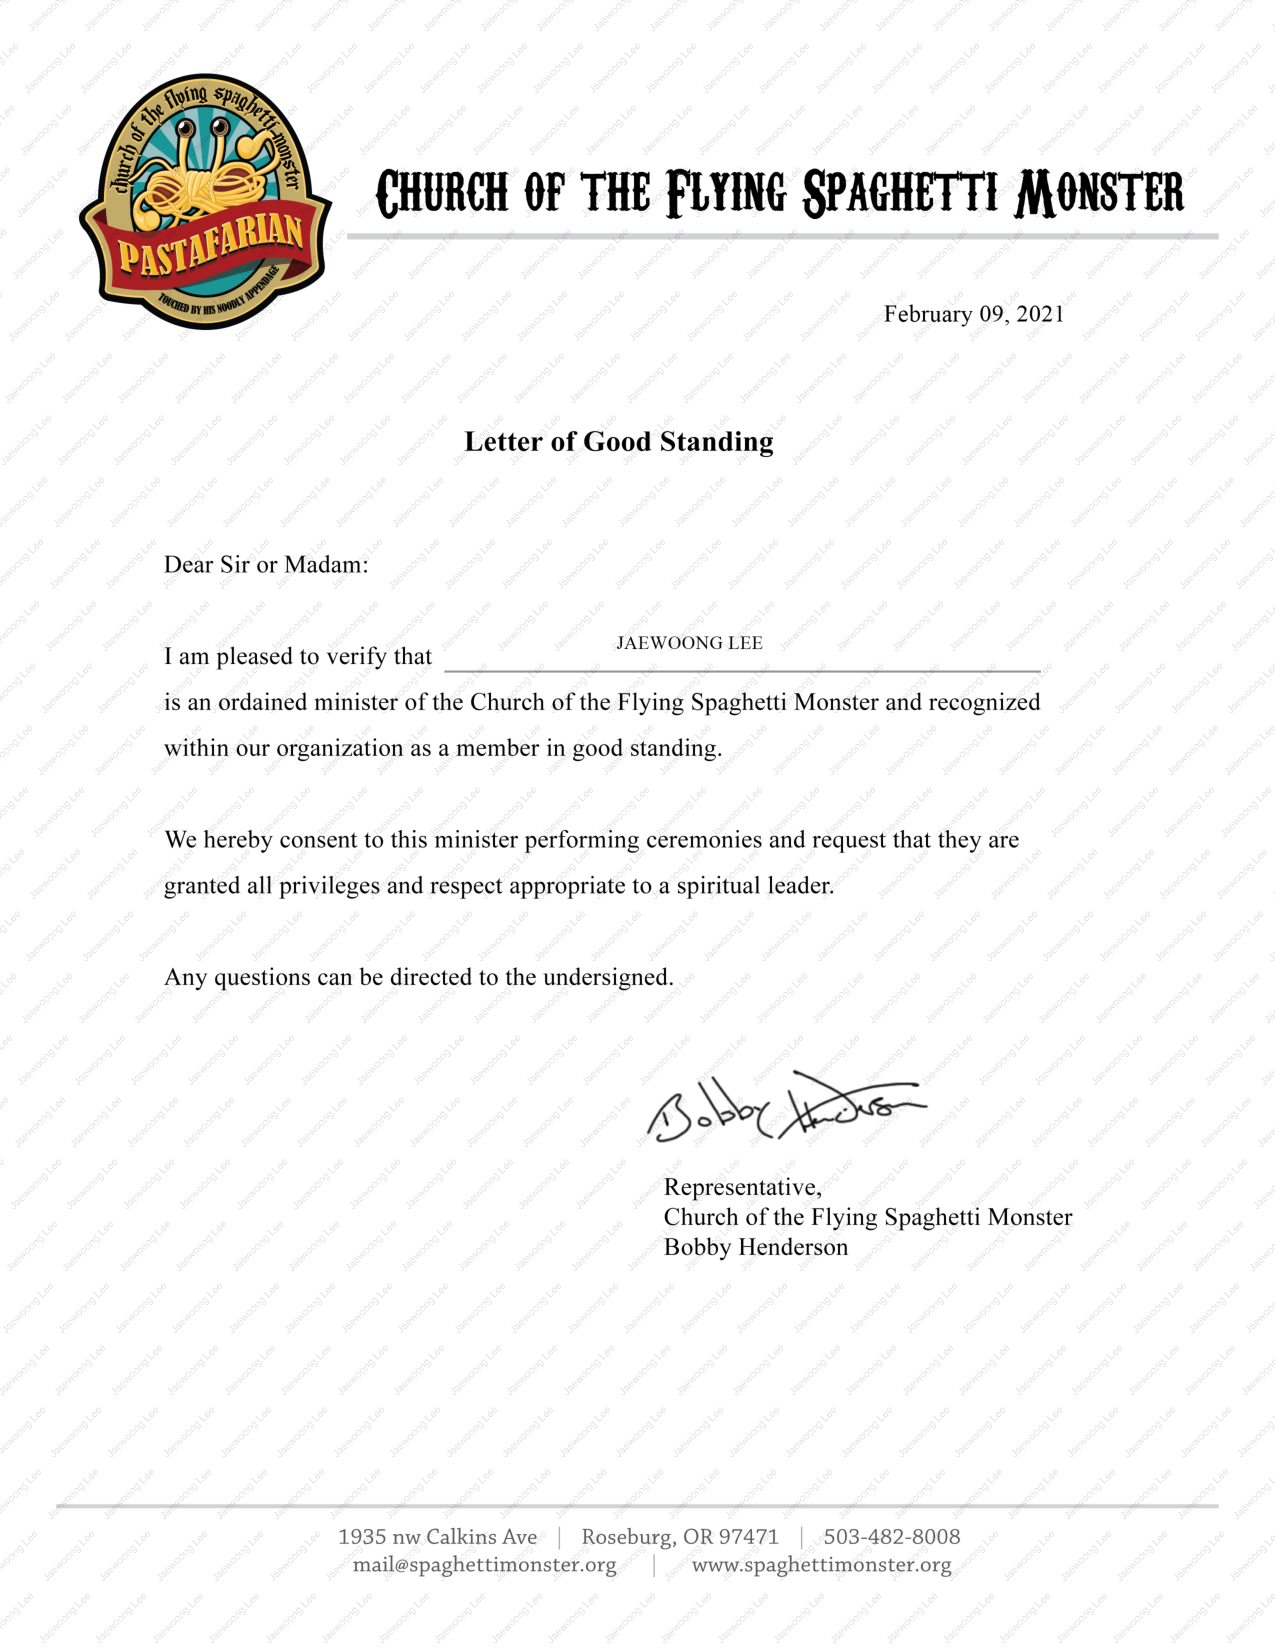
\includepdf[fitpaper= true, pages=-]{Documents/example.pdf}

% [Confirmation of thesis approval]
% add the certificate signed by your committee in a PDF file
% Put your pdf with the filename below, and uncomment it.
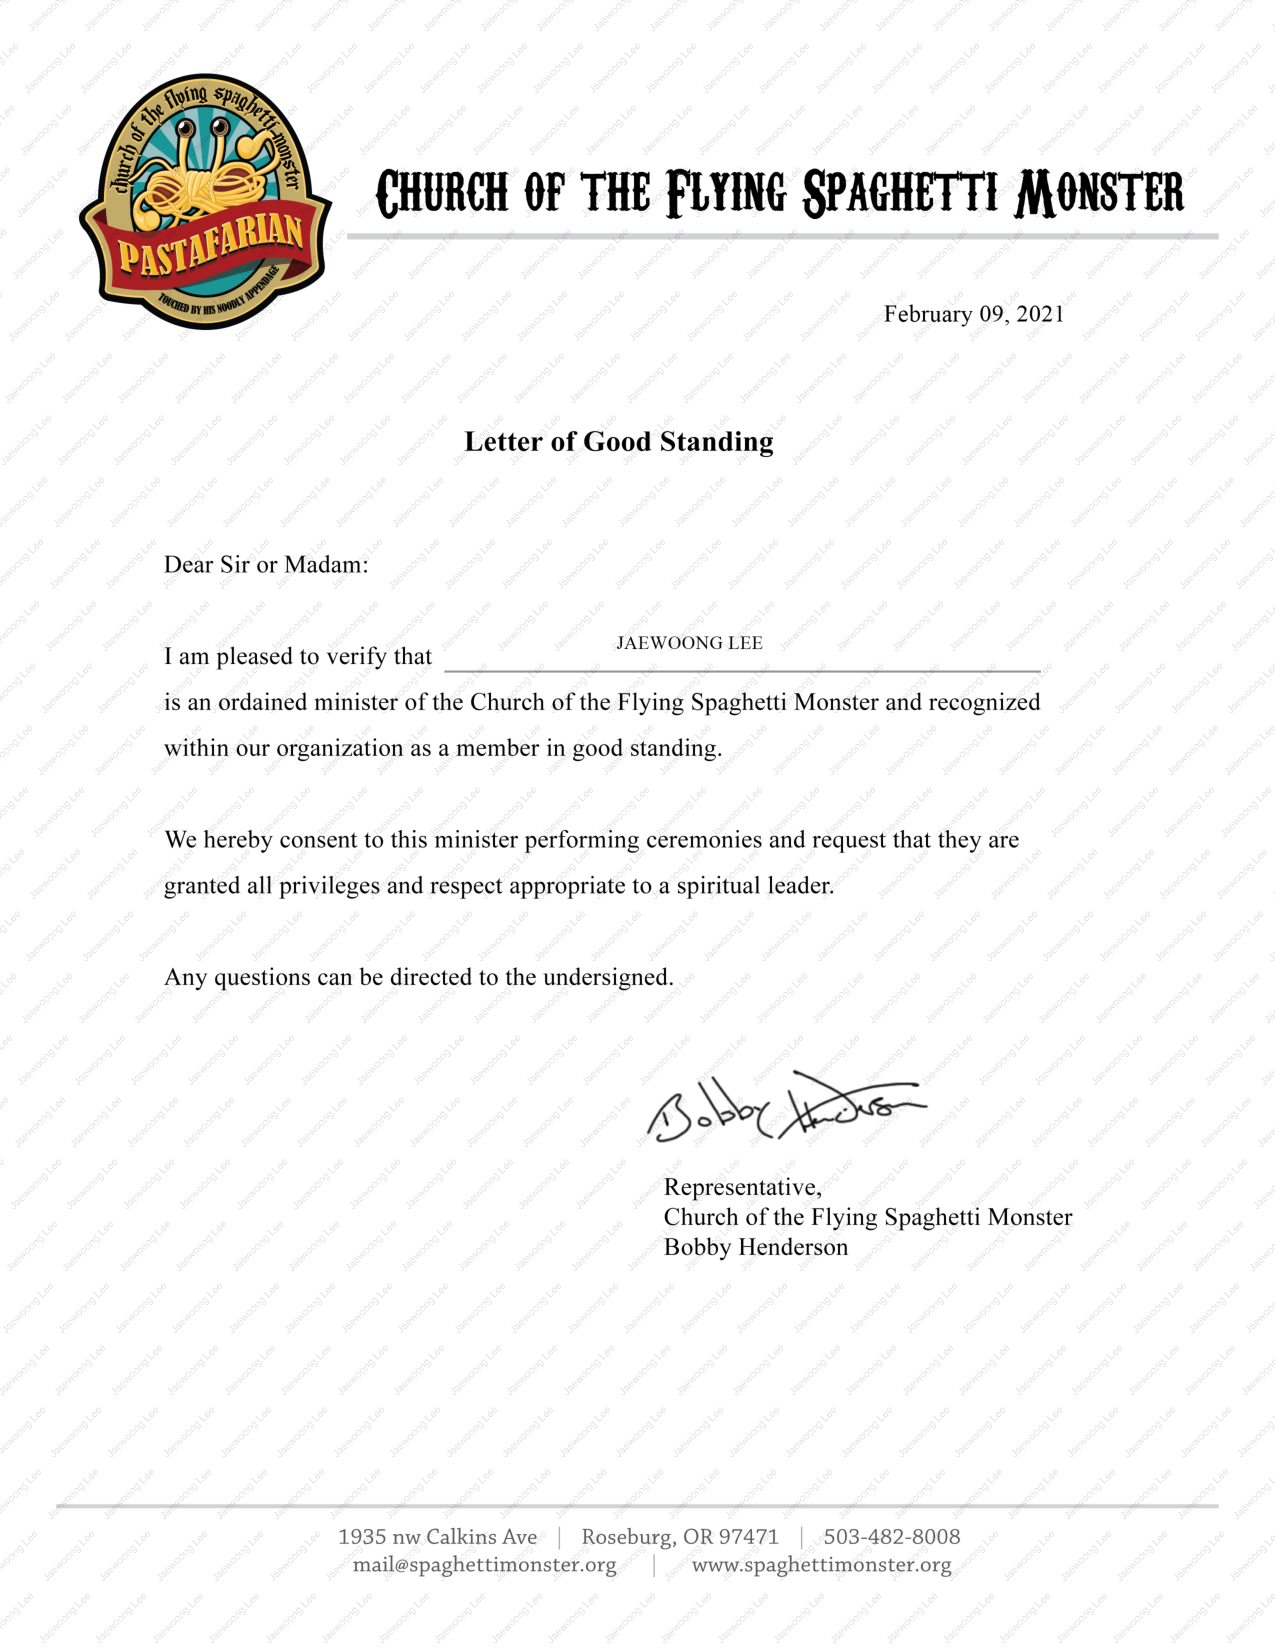
\includepdf[fitpaper= true, pages=-]{Documents/example.pdf}

% Abstract
    \begin{abstract}
    Your abstract should be here. \vfill
    \end{abstract}
    \clearpage

% Do not touch the below 20 lines
\hbox{ }
\thispagestyle{empty}
\clearpage

%%% Table of Contents
\tableofcontents{}
\thispagestyle{empty}
\vfill
\clearpage

%%% List of Figures
\listoffigures{}
\thispagestyle{empty}
\clearpage

%%% List of Tables
\listoftables{}
\thispagestyle{empty}
\clearpage

%%% reset page numbering
\setcounter{page}{1}
%  Do not touch the above 20 lines

    \section*{List of Abbreviations}
    \printacronyms[display=all, heading=none]
    \newpage

    \section{Abstract}

    \textbf{This doctoral dissertation is an addition based on the following papers that the author has already published:}
    \begin{itemize}
        \item \input{Documents/PTB.txt} \nocite{PTB-JW-1}
    \end{itemize}
    \newpage

    \section{Predicting preterm birth using machine learning techniques in oral microbiome}
        \label{section:PTB}

        \textbf{This section includes the published contents:} \\
        \input{Documents/PTB.txt} \nocite{PTB-JW-1}

        \subsection{Introduction}
            Preterm birth (PTB), defined as delivery of newborns before 37 weeks of gestation, is a leading cause of morbidity and mortality in neonates \cite{PTB-rate-1}. Established risk factors for PTB include genitourinary tract infections, short cervical length, and multiple pregnancies \cite{PTB-cause-1}. However, there is still disagreement regarding the magnitude of these factors’ effects on birth outcomes. Early identification of pregnant women at high risk of PTB can facilitate the implementation of strategies to prolong gestation and improve birth outcomes \cite{PTB-care-1}.

            Despite increased understanding of risk factors contributing to PTB, there remains a considerable lack of sensitivity in predictive models that can serve as a framework for intervention strategies \cite{PTB-prediction-1}. Numerous attempts have been made to predict PTB using machine learning techniques combined with data from health records, inflammatory markers, and vaginal microbiome \cite{PTB-prediction-2}. Fetal fibronectin is widely used clinically due to its affordability and simplicity. However, it has a low prediction rate with a sensitivity of only 56\% \cite{PTB-prediction-3}. Cervical length measurement also has limitations due to the hassle and inaccuracy of the procedure and the need for a skilled specialist \cite{PTB-prediction-4}.

            Approximately 70\% of PTBs result from spontaneous onset of preterm labor and preterm pre-labor rupture of membranes (PROM) due to intrauterine infection and inflammation \cite{PTB-prediction-5}. However, the mechanism of PTB cannot be fully explained by inflammatory and infectious pathways as anti-inflammatory and antibiotic treatments could not reduce PTB incidence rates \cite{PTB-mechanism-1}. With advancements in molecular genetic technology, studies on maternal microbiomes using 16S ribosomal RNA (rRNA) sequencing have emerged to explore unknown pathways of PTB \cite{PTB-mechanism-2}.

            Microorganisms associated with PTB have been postulated to originate from one of two places: the reproductive or genitourinary tract ascending through the cervix or a hematogenous route \cite{PTB-mechanism-3}. Recent research has identified vaginal microbial signatures in women who later experience PTB and attempted to predict PTB using cervicovaginal fluid \cite{PTB-mechanism-4}. Although existing reports have verified a potential relationship of vaginal microbiome with PTB, they can only explain an ascending route.

            Decades of epidemiological research studies have suggested that periodontitis is an independent risk factor for various adverse birth outcomes, including PTB \cite{PTB-mechanism-5}. Based on these precedents, it is expected that the oral microbiome can explain another hematogenous route. However, prenatal oral microbiome is not well understood.

            Thus, this study aimed to compare oral microbiome compositions between a PTB group and a full-term birth group, to identify oral microbiome associated with PTB, and to develop a machine learning prediction model of PTB based on oral microbiome compositions.
        \newpage

        \subsection{Materials and methods}
            \subsubsection{Study design and participants}
                This study was conducted on singleton pregnant women admitted for delivery at Jeonbuk National University Hospital between 2019 and 2021. This study received approval from the Ethical Research Committee (IRB file No. 2019-01-024). All participants provided written informed consent. Eligible participants included women admitted for induction delivery, elective cesarean section, and those who were hospitalized due to symptoms of preterm labor or preterm pre-labor rupture of membranes.

            \subsubsection{Data collection and grouping}
                Data on current and historical pregnancy outcomes were collected from questionnaires and electronic medical records. This information encompassed demographic factors (gestational age, birth weight, sex) and maternal risk factors (maternal age at delivery, cesarean section, preterm pre-labor rupture of membranes, previous preterm delivery history, gestational or overt diabetes mellitus, pregnancy-induced or chronic hypertension, and pre-pregnancy overweight or gestational weight gain). All subjects were divided into a PTB group or a full-term birth (FTB) group, with PTB defined as delivery before 37 weeks of gestation.

            \subsubsection{Oral microbiome sample collection}
                Oral microbiome samples were collected using mouthwash within 24 h before delivery. Standard sterile techniques were employed. Medical staff supervised all sample collection procedures. Participants were instructed to avoid brushing their teeth, eating, or drinking 30 min before sampling. Saliva samples were obtained by rinsing the mouth with 12 mL of a gargle solution (E-zen Gargle, JN Pharm, Pyeongtaek, Korea) for 30 s. Sample were labeled with the subject’s anonymous ID and stored at 4 °C until further processing. The resuspended sample was transferred to a microcentrifuge tube. Genomic DNA was extracted using an ExgeneTM Clinic SV kit (GeneAll Biotechnology, Seoul, Korea) according to the manufacturer’s instructions and stored at -20 \textcelsius.

            \subsubsection{16s rRNA gene sequencing and taxonomy assignment}
                Specimens were sent to Department of Biomedical Engineering, Ulsan National Institute of Science and Technology for taxonomy assignment. Then 16S rRNA sequencing was performed using an Illumina MiSeq Reagent Kit v3 (Illumina, San Diego, CA, USA) commissioned by Macrogen (Macrogen, Seoul, Korea). Library protocols for amplifying V3 and V4 regions were used. Pooled library was sequenced using a v3 600 cycle chemistry after diluting the sample to a final concentration of 6 pM with 20\% PhiX control to generate 300 bp paired end reads.

            \subsubsection{Bioinformatics and statistical analysis}
                Independent t-test and chi-square test were used to compare differences between the PTB group and the FTB group. SPSS (version 20.0) was used for all data analyses \cite{SPSS-1}. Statistical significance was considered at $p < 0.05$.

                16S rRNA sequences from study subjects were imported with QIIME2 (version 2022.2) for further processing \cite{QIIME2-1}. Sequences were filtered with DADA2 \cite{DADA2-1}. Amplicon sequence variants (ASV) were assigned taxonomy with the Human Oral Microbiome Database (version 15.22) \cite{HOMD-1}. To measure richness of microbiomes, two diversity indices were calculated. Alpha diversity, a measure of species within a particular community, was calculated using the Faith’s phylogenetic diversity (Faith PD) index within the QIIME2 platform. Communities numerically dominated by a few species will exhibit a low Faith PD index, whereas communities in which abundance is distributed equally among species will exhibit a high evenness. Mann–Whitney–Wilcoxon test was used to find statistically significant differences in Faith PD index. Beta diversity measures dissimilarity between pairs of communities. It was calculated using the Hamming diversity index. PERMANOVA multivariate test was used to calculate statistically significant differences in the Hamming diversity index.

                To identify differentially abundant taxa (DAT) with distinct abundance differences between the PTB group and the FTB group, DESeq2 was implemented using \texttt{DESeqDataSetFromMatrix} method as described in the package tutorial \cite{DESeq2-1}. Taxa with $| \log _2 \textrm{FoldChange} |$ $>$ 1 and adjusted $p < 0.05$ are considered as significant different.

            \subsubsection{Machine learning prediction model development}
                Following qualitative and quantitative analyses of associations between the PTB group and each bacterium, a random forest classifier was used to find the criteria to predict PTB with oral microbiome data. Random forest classification is an ensemble machine learning algorithm that summarizes many decision trees to improve classification evaluations and robustness \cite{RF-1}. Random forest classifier was implemented to predict PTB based on oral microbiome compositions. To assure consistence and reliable classification results \cite{Kfold-1}, we performed stratified $k$-fold cross-validation ($k=5$). Moreover, to decide the best features that could maximize classification evaluations, we performed random forest classification evaluations only with some DAT selected by their importances. Evaluations for classification included accuracy (ACC), balanced accuracy (BA), precision (PRE), sensitivity (SEN), and specificity (SPE).

            \subsubsection{Ethics approval and consent to participate}
                The research protocol was approved by the Institutional Review Board of Jeonbuk National University Hospital (No. 2019-01-024) and was performed according to the Declaration of Helsinki \cite{Helsinki-1}.
        \newpage

        \subsection{Results}
            \subsubsection{Study participant demographics}
                In this study, a total of 69 volunteer mothers were initially recruited. However, one participant with incomplete data and nine individuals with twin pregnancies were excluded from the study cohort. As a result, 59 women (30 in the PTB group and 29 in the FTB group) were included in the final analysis. Demographic and clinical characteristics of subjects in the PTB group and the FTB group are summarized in Table \ref{tab:PTB-clinical}. Because PROM is a major cause of preterm birth, it was significantly higher in PTB group. There was no significant difference in other maternal clinical characteristics between the PTB group and the FTB group. There were no cases with a history of smoking or concurrent periodontal disease in both groups.

            \subsubsection{Comparison of oral microbiomes}
                The oral microbiome comprised 13,953,804 sequences from 59 oral microbiome samples, with 102,305.95 $\pm$ 19,095.60 and 64,823.41 $\pm$ 15,841.65 reads per sample before and after filtering low-quality reads and trimming extra-long tails, respectively. After filtering low-quality reads and trimming extra-long tails, remaining representative reads were clustered in ASVs with their exact sequence match. There were no significant differences in measures of alpha diversity (Faith PD) and beta diversity (Hamming distance) indices for samples between the PTB group and the FTB group (Figure \ref{fig:PTB-diversity}).

                Of 465 genera and species analyzed, 32 DAT between the PTB group and the FTB group were selected by DESeq2 \cite{DESeq2-1}, including 26 FTB-enriched DAT and six PTB-enriched DAT. In order to mitigate the confounding effect of PROM, we excluded 7 PROM-related DATs from these 32 DAT (Figure \ref{fig:PTB-volcano}). There were a total of 25 DATs between the PTB group and the FTB group, with 22 DATs enriched in the FTB group and three in the PTB group, as depicted in Figure \ref{fig:PTB-DAT}.

                Figure \ref{fig:PTB-composition} displays DAT volcano plot in the oral microbiome sorted by differences between FTB-enriched DAT and PTB-enriched DAT proportions, indicating a decrease in gestational age for FTB-enriched DAT proportions. Pearson correlation analysis revealed a strong negative correlation ($r = -0.542$ and $p = 7.8\textrm{e}-6$) between gestational age and difference between PTB-enriched DAT and FTB-enriched DAT proportions.

            \subsubsection{Random forest classification}
                Random forest classifiers were established to classify PTB based on DAT. The best balanced accuracy (0.765 $\pm$ 0.071) was achieved using the nine most important taxa (Figure \ref{fig:PTB-ML}a). The Random forest model calculated the importance of each DAT (Figure \ref{fig:PTB-ML}b). Overall accuracy, precision, sensitivity, and specificity were 0.714 $\pm$ 0.061, 0.700 $\pm$ 0.194, 0.728 $\pm$ 0.058, and 0.743 $\pm$ 0.138, respectively. In order to validate the performance of our machine learning prediction model, we conducted a validation test on 9 twin pregnancies that were excluded from the paper (Figure \ref{fig:PTB-validation}). On PTB subjects of these twin samples, the machine learning classifications have 87.5\% accuracy, comparable to the machine learning classification on the singleton study subjects.

            \begin{table}[p]
                \centering

                \caption[Baseline clinical characteristics of study subjects]{\textbf{Baseline clinical characteristics of study subjects}. Continuous variables: Mean $\pm$ standard deviation. Categorical variables: count (proprotion). Continuous variable for independent $t$-test. Categorical variable for Pearson’s $\chi$-square test.}
                \label{tab:PTB-clinical}
            \end{table}
            \clearpage

            \begin{figure}[p]
                \centering
                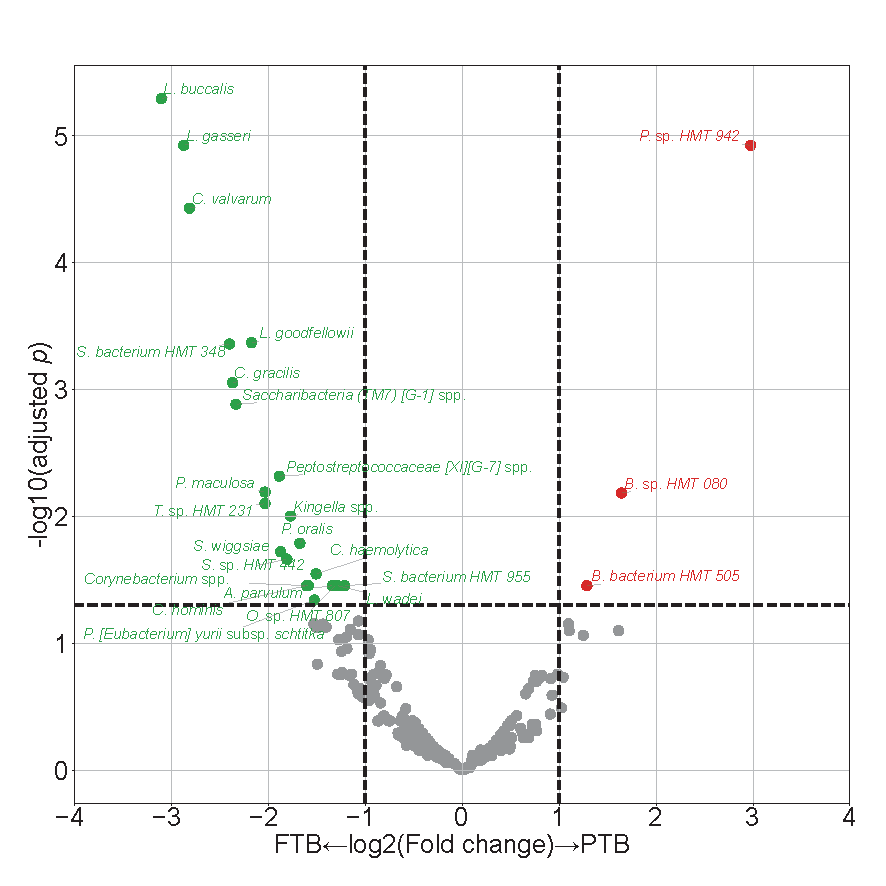
\includegraphics[width=12 cm]{Figures/PTB/Fig1-DAT.pdf}
                \caption[DAT volcano plot]{\textbf{DAT volcano plot}. DAT volcano plot shows DAT, with PTB-enriched DAT shown as red dots and FTB-enriched DAT shown as green dots. Taxa with $| \log _2 \textrm{FoldChange} |$ $>$ 1 and adjusted $p < 0.05$ are considered as significant different.}
                \label{fig:PTB-DAT}
            \end{figure}
            \clearpage

            \begin{figure}[p]
                \centering
                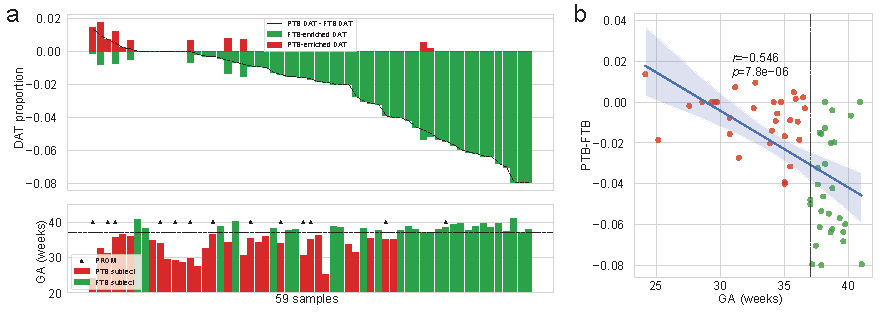
\includegraphics[width=15 cm]{Figures/PTB/Fig2-Composition.pdf}
                \caption[Oral microbiome compositions over DAT]{\textbf{Oral microbiome compositions over DAT}. \textbf{(a)} Proportions of DAT of study subjects. Samples are sorted by difference between PTB-enriched DAT proportion and FTB-enriched DAT proportion. GA of samples are shown, matched with order of upper panel. PTB: red bar, FTB: green bar. PROM: arrow head. \textbf{(b)} Correlation plot with GA and difference between PTB-enriched DAT proportion and FTB-enriched DAT proportion. Pearson correlation shows strong negative coefficient ($r = -0.542$ and $p = 7.8e-06$) between GA and difference between PTB-enriched DAT proportion and FTB-enriched DAT proportion.}
                \label{fig:PTB-composition}
            \end{figure}
            \clearpage

            \begin{figure}[p]
                \centering
                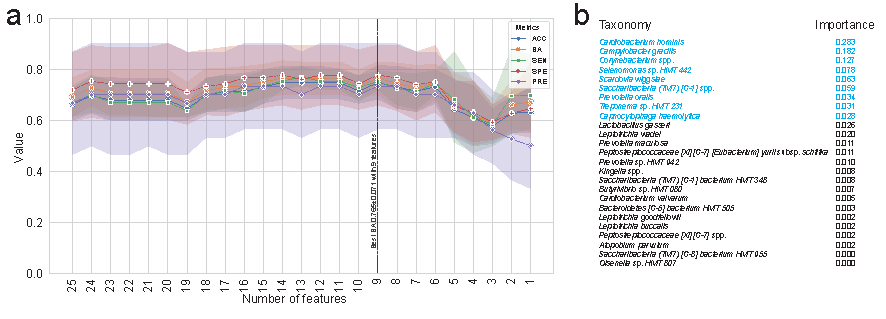
\includegraphics[width=15 cm]{Figures/PTB/Fig3-ML.pdf}
                \caption[Machine learning evaluations over DAT]{\textbf{Machine learning evaluations over DAT}. \textbf{(a)} Machine learning evaluation upon number of features (DAT). Random Forest classifier has the best balanced accuracy (mean $\pm$ standard deviation.; 0.765 $\pm$ 0.071) with the nine most important DAT. \textbf{(b)} Importance of DAT is shown. Note that 0 $\le$ importance $\le$ 1, and $\sum$ importance $=$ 1. The 20 most important DAT that give the best balanced accuracy is marked with blue.}
                \label{fig:PTB-ML}
            \end{figure}
            \clearpage

            \begin{figure}[p]
                \centering
                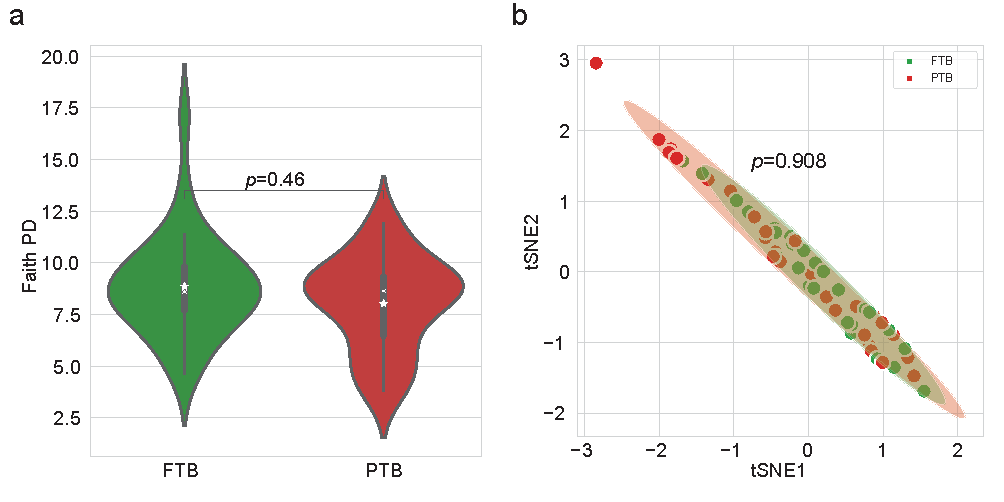
\includegraphics[width=15 cm]{Figures/PTB/FigS1-Diversity.pdf}
                \caption[Diversity indices]{\textbf{Diversity indices}. \textbf{(a)} Alpha diversity index (Faith PD). Mann-Whitney-Wilcoxon test did not find statistically significant difference between the PTB group and the FTB group. Mean values are marked with star-point. \textbf{(b)} t-SNE plot with beta diversity index (Hamming distance). PERMANOVA multivariate test did not find statistically significant difference between the PTB group and the FTB group.}
                \label{fig:PTB-diversity}
            \end{figure}
            \clearpage

            \begin{figure}[p]
                \centering
                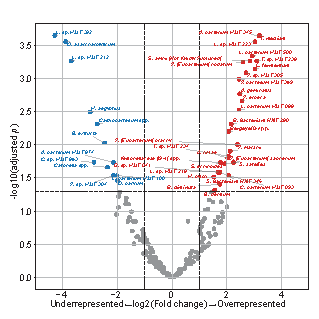
\includegraphics[width=12 cm]{Figures/PTB/FigS2-PROM.pdf}
                \caption[PROM-related DAT volcano plot]{\textbf{PROM-related DAT volcano plot}. This is a subgroup analysis between 12 participants in PTB group with PROM and 18 participants in PTB group without PROM, 42 PROM-related DAT were selected between these two groups. Out of these 42 PROM-related DAT, only 7 DAT overlapped with PTB-related DAT, as it indicated by the bold marking. Volcano plot shows PROM-related DAT, with 12 PROM-underrepresented DAT shown as blue dots and 30 PROM-overrepresented DAT shown as red dots. Taxa with $| \log _2 \textrm{FoldChange} |$ $>$ 1 and adjusted $p < 0.05$ are considered as significant different.}
                \label{fig:PTB-volcano}
            \end{figure}
            \clearpage

            \begin{figure}[p]
                \centering
                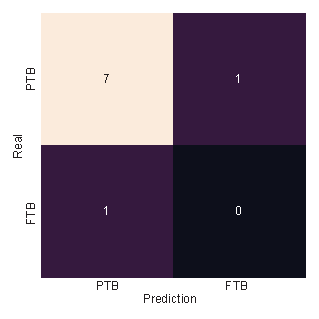
\includegraphics[width=12 cm]{Figures/PTB/FigS3-validation}
                \caption[Heatmap plot of PTB classification with validation data]{\textbf{Heatmap plot of PTB classification with validation data}. A validation test on 9 twin pregnancies that had excluded from the paper was conducted. They consist of 8 PTB subjects and 1 FTB subject. As twin pregnancies have a 7-10 times higher PTB rate than singleton pregnancies, resulting in a majority of the test data falling into the PTB group. The machine learning classifications have 87.5\% accuracy, comparable to the machine learning classification on the singleton study subjects (Mean $\pm$ standard deviation. 0.714 $\pm$ 0.061)}
                \label{fig:PTB-validation}
            \end{figure}
            \clearpage
        \newpage

        \subsection{Discussion}
            In this study, we developed a method for predicting PTB based on random forest classifier using oral microbiome compositions. Recently, several sporadic reports have suggested a bidirectional relationship between oral microbiome and pregnancy \cite{PTB-mechanism-3}. However, prenatal oral microbiome is not well understood yet. Some research has shown that oral microbial dysbiosis combined with gingival inflammation can lead to adverse pregnancy  outcomes, including low birth weight, PTB, pre-eclampsia, and miscarriages \cite{PTB-mechanism-6}. Nevertheless, these results have been inconsistent due to methodologies employed in studies that only target known pathogens.

            \textit{Fusobacterium nucleatum} is the most prevalent oral microbiome studied. \textit{Fusobacterium nucleatum} is a Gramnegative, anaerobic, filamentous oral microbiome. It is considered one of the most abundant species in the oral microbiome. It can also be isolated from vaginal microbiome \cite{PTB-mechanism-7, PTB-mechanism-8}.
        \newpage

    \section{Periodontitis}
        \label{section:Periodontitis}
        \subsection{Introduction}
        \newpage

        \subsection{Materials and methods}
        \newpage

        \subsection{Results}
        \newpage

        \subsection{Discussion}
        \newpage

    \section{General conclusion and future perspective}
        \label{section:conclusion}
        \subsection{General conclusions}
            In conclusion, the research described in this doctoral dissertation was conducted to identify significant ...

            In the Section \ref{section:PTB}, I show that
        \newpage

        \subsection{Plan for future}
        \newpage

        \subsection{Future perspective}
        \newpage

% Reference
    \addcontentsline{toc}{section}{References}
    \bibliographystyle{apacite}
    \bibliography{references.bib}
    \clearpage

% Acknowledgements
    \addcontentsline{toc}{section}{Acknowledgments}
    \section*{\hfill \Large Acknowledgments \hfill}
        I would like to disclose my earnest appreciation for my advisor, Professor Semin Lee, who provided solicitous supervision and cherished opportunities throughout the course of my research. His advice and consultation encouraged me to become as a researcher and to receive all humility and gentleness. I am also grateful to all of my committee members, Professor AAA, Professor BBB, Professor CCC, and Professor DDD, for their critical and meaningful mentions and suggestions.

        I extend my deepest gratitude to my Lord, \textit{the Flying Spaghetti Monster}, His Noodly Appendage has guided me through the twist and turns of this academic journey. His presence, ever comforting and mysterious, has been a source of strength and humor during both highs and lows. In moments of doubt, I found solace in the belief that you were there, gently reminding me to keep fiath in the process. His Holy Noodle has nourished my mind, and for that, I am truly overwhelmed. May His Holy Noodle continue to guide me in all my future endeavors. R'Amen.

        (Professors)

        I would like to extend my heartfelt gratitude to my colleagues of the Computational Biology Lab, whose collaboration, friendship, brotherhood, and support have been an invaluable part of my journey. Your willingness to share insights, engage in thoughtful discussions, and offer encouragement during the challenging moments of research has significantly shaped my academic experience. The camaraderie in the Computational Biology Lab made even the most demanding days more enjoyable, and I am deeply grateful for the collaborative environment we created together. I appreciate you for standing by my side throughout this Ph.D. journey.

        I would like to express my heartfelt gratitude to my family, whose unwavering support has been the foundation of everything I have achieved. Your love, encouragement, and belief in me have sustained me through every challenge, and I could not have come this far without you. From your words of wisdom to your patience and understanding, each of you has played a vital role in helping me navigate this journey. The strength and comfort I have drawn from our family bond have been my greatest source of resilience. Your presence, both near and far, has filled my life with warmth and motivation. I am deeply grateful for your unconditional love and for always being there when I needed you the most. Thank you for being my constant source of strength and inspiration.

        I am incredibly pleased to my friends, especially my GSHS alumni, for their unwavering support and encouragement throughout this journey. The bonds we formed back in our school days have only grown stronger over the years, and I am fortunate to have had such loyal and understanding friends by my side. Your constant words of motivation, and even moments of levity during stressful times have helped keep me grounded. Whether it was a late-night conversations, a shared laugh, or a simple message of reassurance, you all have played a vital role in keeping me focused and motivated. I am relieved for the ways you celebrated each small achievement with me and how you patiently listened to my worries. The memories of our shared past provided me with comfort and a sense of stability when the road ahead felt uncertain. I could not have reached this point without the love and friendship that you all have generously given. Each of your, in your unique way, has contributed to this dissertation, even if indirectly, and for that, I am forever beholden. I look forward to continuing our friendship as we all grow in our individual paths, knowing that the support we share is something truly special.

        I would like to express my sincere gratitude to the amazing members of my animal protection groups, DRDR and UNIMALS, whose dedication and compassion have been a constant source of motivation. Your unwavering commitment to improving the lives of animals has inspired me throughout this journey. I am also thankful for the beautiful cats we have cared for, whose presence brought both joy and purpose to our allegiance. Their playful spirits and gentle companionship served as daily reminders of why we continue to fight for animal rights. The bond we share, both with each other and with the animals we protect, has enriched my life in countless ways. I appreciate you all again for your support, dedication, and for being part of this meaningful cause.

        I would like to express my deepest gratitude to everyone I have had the honor of meeting throughout this journey. Your kindness, encouragement, and support have carried me through both the challenging and rewarding moments of my life. Whether through a kind word, thoughtful advice, or simply being there when I needed it most, your presence has made all the difference. I am incredibly fortunate to have received such generosity and warmth from those around me, and I do not take it for granted. Every act of kindness, no matter how big or small, has been a source of strength and motivation for me. To all my friends, colleagues, mentors, and beloved ones, thank you for your unwavering support. I am truly grateful for each of you, and your kindness has left an indelible mark on my journey.

        \begin{center}
            My Lord, \textit{the Flying Spaghetti Monster},\\
            give us grace to accept with serenity the things that cannot be changed,\\
            courage to change the things that should be changed,\\
            and the wisdom to distinguish the one from the other.

            \medspace

            Glory be to \textit{the Meatball}, to \textit{the Sauce}, and to \textit{the Holy Noodle}. \\
            As it was in the beginning, is now, and ever shall be. \\
            R'Amen.
        \end{center}
    \clearpage

%%% The following page is intentionally left as blank
% White attachment form
\hbox{ }
\thispagestyle{empty}
\clearpage
\end{document}